Space Vector Pulse Width Modulation (SVPWM) is a sophisticated modulation
technique commonly used in three-phase inverters. It is designed to generate an
output voltage waveform with precise control over both amplitude and frequency.
SVPWM achieves this by synthesizing the output voltage using a combination of
eight fundamental voltage vectors. These vectors include one "zero sequence
vector," which represents a state where all three inverter legs are switched to
the same state, and six "active vectors," which correspond to states where the
inverter legs are switched to create specific voltage differences between the
phases.

\subsection{Basic Voltage Vectors}
SVPWM utilizes eight basic voltage vectors, which are combinations of
magnitudes and directions of the voltage vectors in the abc reference frame.
These vectors are represented as $V_0$ through $V_7$ . Each vector corresponds
to a unique combination of switching states for the three inverter legs (a, b,
and c). Figure \ref{fig:combined} outline these basic voltage vectors.\\
\begin{figure}[ht]
    \centering
    \begin{subfigure}[b]{0.45\textwidth}
        \centering
        \resizebox{\linewidth}{!}{
            \begin{tikzpicture}[auto, node distance=2cm, >=latex']
                % Define the origin
                \coordinate (O) at (0,0);

                % Define the vectors
                \coordinate (V1) at ({3*cos(0)},{3*sin(0)});
                \coordinate (V2) at ({3*cos(60)},{3*sin(60)});
                \coordinate (V3) at ({3*cos(120)},{3*sin(120)});
                \coordinate (V4) at ({3*cos(180)},{3*sin(180)});
                \coordinate (V5) at ({3*cos(240)},{3*sin(240)});
                \coordinate (V6) at ({3*cos(300)},{3*sin(300)});

                % Draw the vectors
                \draw[->, thick] (O) -- (V1) node[midway, above,pos=1] {$\mathbf{V_1}$};
                \draw[->, thick] (O) -- (V2) node[midway, above,pos=1] {$\mathbf{V_2}$};
                \draw[->, thick] (O) -- (V3) node[midway, above,pos=1] {$\mathbf{V_3}$};
                \draw[->, thick] (O) -- (V4) node[midway, above,pos=1] {$\mathbf{V_4}$};
                \draw[->, thick] (O) -- (V5) node[midway, below,pos=1] {$\mathbf{V_5}$};
                \draw[->, thick] (O) -- (V6) node[midway, below,pos=1] {$\mathbf{V_6}$};

                % Draw the axes
                \draw[->] (-4,0) -- (4,0) node[right] {$\alpha$};
                \draw[->] (0,-4) -- (0,4) node[above] {$\beta$};
            \end{tikzpicture}
        }
        \caption{Space Vector}
        \label{fig:SVM}
    \end{subfigure}
    \hfill
    \begin{subfigure}[b]{0.45\textwidth}
        \centering
        \begin{tabular}{|c|c|c|c|c|}
            \hline
            Vector  & \(S_A\) & \(S_B\) & \(S_C\) & Description   \\ \hline
            \(V_0\) & 0       & 0       & 0       & Zero Vector   \\ \hline
            \(V_1\) & 1       & 0       & 0       & Active Vector \\ \hline
            \(V_2\) & 1       & 1       & 0       & Active Vector \\ \hline
            \(V_3\) & 0       & 1       & 0       & Active Vector \\ \hline
            \(V_4\) & 0       & 1       & 1       & Active Vector \\ \hline
            \(V_5\) & 0       & 0       & 1       & Active Vector \\ \hline
            \(V_6\) & 1       & 0       & 1       & Active Vector \\ \hline
            \(V_7\) & 1       & 1       & 1       & Zero Vector   \\ \hline
        \end{tabular}
        \caption{Possible Switch States for the 8 Space Vectors}
        \label{tab:switch_states}
    \end{subfigure}
    \caption{Space Vector and Switching States}
    \label{fig:combined}
\end{figure}

The vectors can be visualized in a hexagonal plane, where each active vector
represents a specific direction and magnitude in the two-dimensional space of
the voltage waveform. The zero vectors $V_0$ and $V_7$ do not contribute to the
direction but help in controlling the overall voltage magnitude and maintaining
the desired output voltage.\\

Each vector corresponds to specific switching states of the inverter's power
transistors. The switching states determine which transistors are turned on and
off, thereby controlling the flow of current in the three phases.

\begin{enumerate}
    \item \textbf{Zero Vector ($V_0$ and $V_7$)}:These vectors represent a state where all three legs of the inverter are either connected to the positive or negative terminal of the DC bus, resulting in zero voltage output. These are used to control the overall magnitude of the output voltage and provide a zero voltage state during the modulation cycle.
    \item \textbf{Active Vectors ($V_1$ to $V_6$)}:These vectors represent states where two legs are connected to one terminal of the DC bus and one leg to the other terminal. They define the direction and magnitude of the output voltage.
\end{enumerate}

\subsection{Vector Selection}
Given the desired voltage vector in the $\alpha\beta$ plane, the nearest active
vectors are selected to approximate it. This selection is based on the angle
and magnitude of the desired vector relative to the active vectors. The process
involves determining the sector in which the reference voltage vector lies. The
$\alpha\beta$ plane is divided into six sectors, each spanning 60 degrees.\\

Once the sector is identified, the two adjacent active vectors defining this
sector are selected. These vectors are chosen because they are the closest to
the desired voltage vector and can best approximate its position. For example,
if the desired voltage vector lies in the first sector, the active vectors
$V_1$ and $V_2$ are selected. The reference vector is then synthesized by
linearly combining these two active vectors and a zero vector.\\

The zero vectors ($V_0$ and $V_7$) are used to balance the time intervals to
ensure that the total duration of each switching period is maintained. This
selection and combination process ensures that the resulting output voltage
vector closely follows the desired reference vector, minimizing the error and
improving the overall performance of the inverter.

\subsection{Synthesis of Output Voltage}
The output voltage synthesis entails selecting the nearest active vectors to
achieve the desired voltage magnitude and phase angle. This is achieved by
modulating between the closest two active vectors and incorporating a zero
vector as needed.

\subsubsection{Determining the Time Intervals}

\begin{figure}[ht]
    \centering
    \resizebox{0.5\linewidth}{!}{
        \begin{tikzpicture}[auto, node distance=2cm, >=latex']
            % Define the origin
            \coordinate (O) at (0,0);

            % Define the vectors
            \coordinate (V1) at ({6*cos(0)},{6*sin(0)});
            \coordinate (V2) at ({6*cos(60)},{6*sin(60)});
            \coordinate (V1*) at ({4*cos(0)},{4*sin(0)});
            \coordinate (V2*) at ({4*cos(60)},{4*sin(60)});
            \coordinate (VR) at ({4*cos(0)+4*cos(60)},{4*sin(60)+4*sin(0)});

            % Draw the vectors
            \draw[->, thick] (O) -- (VR) node[midway, above,pos=1] {$\mathbf{V_r}$};
            \draw[->, thick] (O) -- (V1) node[midway, above,pos=1] {$\mathbf{V_1}$};
            \draw[->, thick] (O) -- (V2) node[midway, above,pos=1] {$\mathbf{V_2}$};
            \draw[->, thick] (O) -- (V1*) node[midway, above left,pos=1] {$\mathbf{V_1'}$};
            \draw[->, thick] (O) -- (V2*) node[midway, left,pos=1] {$\mathbf{V_2'}$};

            % Draw Projections
            \draw[->, dashed] (V1*) -- (VR);
            \draw[->, dashed] (V2*) -- (VR);

            % Draw Arc
            \draw (2,0) arc[start angle=0, end angle=30, radius=2] node[midway, right] {$\theta$};

        \end{tikzpicture}
    }
    \caption{Time Interval Calculation}
    \label{fig:til}
\end{figure}

Given the vector \( V_r \), represented by \( V_1 \) and \( V_2 \), the
normalized time durations \( T_A \) and \( T_B \) are calculated as follows:
\[
    V_1' = V_1 \frac{T_A}{T_s}
\]
\[
    V_2' = V_2 \frac{T_B}{T_s}
\]
Using the sine law:
\[
    \frac{V_1'}{\sin \left(\frac{\pi}{3} - \theta\right)} = \frac{V_2'}{\sin \theta} = \frac{V_r}{\sin \frac{2\pi}{3}}
\]
\[
    \frac{V_1 T_A}{\sin \left(\frac{\pi}{3} - \theta\right)} = \frac{V_2 T_B}{\sin \theta} = \frac{V_r T_s}{\sin \frac{2\pi}{3}}
\]
\[
    T_A = \frac{V_r}{V_1} \frac{2}{\sqrt{3}} T_s \sin \left(\frac{\pi}{3} - \theta\right)
\]
\[
    T_B = \frac{V_r}{V_2} \frac{2}{\sqrt{3}} T_s \sin \theta
\]
Magnitude of \( V_1 = V_2 = \frac{2}{3} V_D \)

\noindent
In normalized units, where \( M = \frac{\sqrt{3} V_r T_s}{V_D} \):
\[
    T_A = M \sin \left(\frac{\pi}{3} - \theta\right)
\]
\[
    T_B = M \sin \theta
\]
\( M \) is the modulation index.

\noindent
For the \( N \)-th Sector, \( \theta \rightarrow \theta - (N-1) \frac{\pi}{3}
\):
\[
    T_A = M \sin \left(\frac{N \pi}{3} - \theta\right)
\]
\[
    T_B = M \sin \left(\left(-(N-1) \frac{\pi}{3}\right) + \theta\right)
\]

\subsubsection{Switching Sequence}
Implementing a switching sequence that minimizes switching losses and ensures
smooth transitions between vectors is crucial for the efficiency and
performance of SVPWM. This sequence involves switching between the active and
zero vectors in a manner that reduces the number of switching operations and
distributes the switching events evenly across the phases.\\

The primary goal is to minimize the number of times the switches in the
inverter change states, which helps in reducing switching losses. By doing so,
the overall efficiency of the inverter improves, and the heat generated by
switching operations is minimized. The secondary goal is to ensure that the
transitions between the voltage vectors are smooth, which helps in maintaining
a high-quality output voltage waveform with minimal harmonic distortion.

\begin{table}[ht]
    \centering
    \begin{tabular}{|c|c|c|c|c|c|}
        \hline
        Sector                  & Sequence      & Active Vector 1 & Zero Vector & Active Vector 2 \\ \hline
        $0^\circ - 60^\circ$    & \text{Case 1} & $V1$            & $V0$        & $V2$            \\ \hline
        $60^\circ - 120^\circ$  & \text{Case 2} & $V2$            & $V0$        & $V3$            \\ \hline
        $120^\circ - 180^\circ$ & \text{Case 3} & $V3$            & $V0$        & $V4$            \\ \hline
        $180^\circ - 240^\circ$ & \text{Case 4} & $V4$            & $V0$        & $V5$            \\ \hline
        $240^\circ - 300^\circ$ & \text{Case 5} & $V5$            & $V0$        & $V6$            \\ \hline
        $300^\circ - 360^\circ$ & \text{Case 6} & $V6$            & $V0$        & $V1$            \\ \hline
    \end{tabular}
    \caption{Switching Sequence for Each Sector}
    \label{tab:switching-sequence}
\end{table}

\subsubsection{Gate Pulse Generation}
The gate pulses are generated in a specific manner to achieve these objectives.
When the inverter bridge transitions through different active vectors, the
switching sequence is designed such that only one of the half-bridges changes
its state at any given time. This is achieved by arranging the active and zero
vectors in a specific order, ensuring that the transitions involve only a
single switch change per half-bridge.\\

To determine the optimal switching sequence, the following steps are taken:

\begin{itemize}
    \item \textbf{Sector Division}:The entire space vector plane is divided into six sectors, each spanning 60 degrees. Each sector has a unique combination of active and zero vectors that are used to synthesize the desired output voltage vector.
    \item\textbf{Case Analysis for Each Sector}: For each of the six sectors, a detailed analysis is performed to arrange the active and zero vectors in an optimal sequence. This involves selecting the nearest active vectors to the desired output vector and arranging them along with the zero vectors in a way that minimizes switching operations.
    \item \textbf{Sequence Arrangement}:The active and zero vectors are arranged in a sequence that ensures only one of the half-bridges changes its state at any time. This typically involves transitioning from an active vector to a zero vector, then to the next active vector, and so on. The specific sequence depends on the position of the desired output vector within the sector.
\end{itemize}

\begin{figure}[ht]
    \centering
    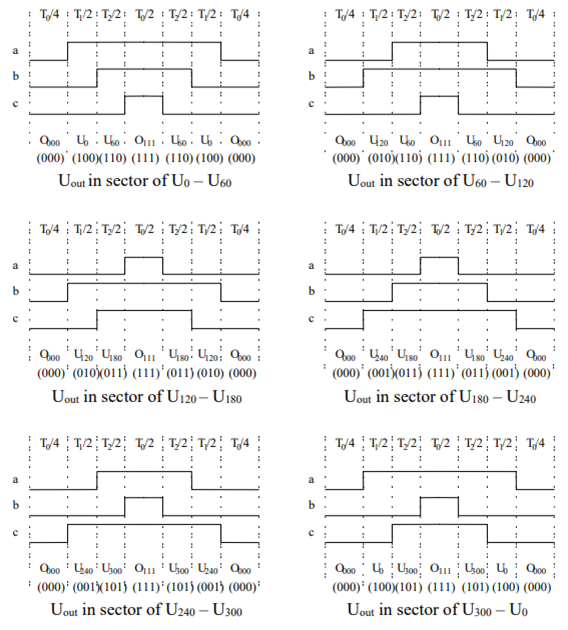
\includegraphics[width=\textwidth]{sequence.png}
    \caption{Gate Pulse Sequence}
    \label{fig:gate_pulse_sequence}
\end{figure}